\documentclass[UTF8,12pt]{article}
\usepackage{ctex}
\usepackage{indentfirst}
\usepackage{color}
\usepackage{hyperref}
\usepackage{graphicx}
\usepackage{subfigure}
\usepackage{pdfpages}
\usepackage{listings}
\hypersetup{
    hidelinks,
	colorlinks=true,
	allcolors=black,
	pdfstartview=Fit,
	breaklinks=true
}

\definecolor{dkgreen}{rgb}{0,0.6,0}
\definecolor{gray}{rgb}{0.5,0.5,0.5}
\definecolor{mauve}{rgb}{0.58,0,0.82}

\lstset{ %
  language=Octave,                % the language of the code
  basicstyle=\footnotesize,           % the size of the fonts that are used for the code
  numbers=left,                   % where to put the line-numbers
  numberstyle=\tiny\color{gray},  % the style that is used for the line-numbers
  stepnumber=2,                   % the step between two line-numbers. If it's 1, each line 
                                  % will be numbered
  numbersep=5pt,                  % how far the line-numbers are from the code
  backgroundcolor=\color{white},      % choose the background color. You must add \usepackage{color}
  showspaces=false,               % show spaces adding particular underscores
  showstringspaces=false,         % underline spaces within strings
  showtabs=false,                 % show tabs within strings adding particular underscores
  frame=single,                   % adds a frame around the code
  rulecolor=\color{black},        % if not set, the frame-color may be changed on line-breaks within not-black text (e.g. commens (green here))
  tabsize=2,                      % sets default tabsize to 2 spaces
  captionpos=b,                   % sets the caption-position to bottom
  breaklines=true,                % sets automatic line breaking
  breakatwhitespace=false,        % sets if automatic breaks should only happen at whitespace
  title=\lstname,                   % show the filename of files included with \lstinputlisting;
                                  % also try caption instead of title
  keywordstyle=\color{blue},          % keyword style
  commentstyle=\color{dkgreen},       % comment style
  stringstyle=\color{mauve},         % string literal style
  escapeinside={\%*}{*)},            % if you want to add LaTeX within your code
  morekeywords={*,...}               % if you want to add more keywords to the set
}


\setlength{\parindent}{2em}

\begin{document}

\begin{center}
    \tableofcontents
\end{center}
\newpage

\section{实验目的与要求}
\subsection{实验目的}
\begin{enumerate}
    \item 掌握C++、JAVA或Python等集成开发环境编写网络程序的方法
    \item 掌握客户/服务器(C/S)应用的工作方式
    \item 学习网络中进程之间通信的原理和实现方法
    \item 要求本机既是客户端又是服务器端
\end{enumerate}
\subsection{实验要求}
网络编程是通过使用套接字来达到进程间通信目的的编程,Socket编程是网络编程的主流工具,Socket API是实现进程间通信的一种编程设施,也是一种为进程间提供底层抽象的机制,提供了访问下层通信协议的大量系统调用和相应的数据结构。本实验利用Socket API编写网络通信程序。

编写一个基于socket的简易聊天程序。所编写的程序应具有如下功能:
\begin{enumerate}
    \item 具有点对点通信功能,任意客户端之间能够发送消息
    \item 具有群组通信功能,客户端能够向组内成员同时发送消息,其他组成员不能收到
    \item 具有广播功能,客户端能够向所有其他成员广播消息
\end{enumerate}
\section{实验原理与实验内容}
\subsection{实验原理}
\subsubsection{点对点通信功能}
实现网络点对点通讯程序的关键步骤就是实现信息在网络中的发送和接收。数据接收使用的是Socket,数据发送使用的是NetworkStream。

实现代码如下:
\begin{lstlisting}[title=利用Socket来接收信息,frame=shadowbox]
    TcpListener tlListen1 = new TcpListener ( 8889 ) ;
      //侦听端口号
      tlListen1.Start ( ) ;
      Socket skSocket = tlListen1.AcceptSocket ( ) ;
      //接受远程计算机的连接请求,并获得用以接收数据的Socket实例
      EndPoint tempRemoteEP = skSocket.RemoteEndPoint  ;
      //获得远程计算机对应的网络远程终结点
      while (  true )
      {
          Byte [] byStream = new Byte[80] ;
          //定义从远程计算机接收到数据存放的数据缓冲区
          int i = skSocket.ReceiveFrom  ( byStream   , ref tempRemoteEP  ) ;
          //接收数据,并存放到定义的缓冲区中
          string sMessage = System.Text.Encoding.UTF8.GetString ( byStream  ) ;
          //以指定的编码,从缓冲区中解析出内容
          MessageBox.Show ( sMessage ) ;
          //显示传送来的数据
      }
\end{lstlisting}

\begin{lstlisting}[title=利用NetworkStream来发送信息,frame=shadowbox]
    TcpClient tcpc = new TcpClient (  "10.138.198.213"  , 8888  ) ;
    //对IP地址为“10.138.198.213”的计算机的8888端口提出连接申请
   NetworkStream tcpStream = tcpc.GetStream ( ) ;
   //如果连接申请建立,则获得用以传送数据的数据流
string sMsg = "您好,见到您很高兴" ;
   StreamWriter reqStreamW = new StreamWriter ( tcpStream  ) ;
   //以特定的编码往向数据流中写入数据 ,默认为UTF8编码
   reqStreamW.Write ( sMsg  ) ;
   //将字符串写入数据流中
   reqStreamW.Flush ( ) ;
   //清理当前编写器的所有缓冲区,并使所有缓冲数据写入基础流
\end{lstlisting}

\subsubsection{群组通信功能}
组播编程需要UDP,有两个类支持组播网络编程Socket和UdpClient。一台计算机要加入某一个组,然后接收发往这个组的信息。Socket类要调用SetSocketOption函数加入和离开某一个组。UdpClient类有直接的加入和离开某个组的成员函数可以调用。而向某个组发信息,则没有什么特殊的,只需把发送数据的目的地址设为组播地址就可以了。

实现代码如下:
\begin{lstlisting}[title=发送端,frame=shadowbox]
    Socket s = new Socket(AddressFamily.InterNetwork, SocketType.Dgram, ProtocolType.Udp);
    IPEndPoint iep = new IPEndPoint(IPAddress.Parse("224.0.0.1"), 3000);
    EndPoint ep = (EndPoint)iep;
byte[] b = Encoding.ASCII.GetBytes("just a test!");
    s.SendTo(b, ep);
    s.Close();
\end{lstlisting}

\begin{lstlisting}[title=接收端,frame=shadowbox]
    Socket s = new Socket(AddressFamily.InterNetwork, SocketType.Dgram, ProtocolType.Udp);
    IPEndPoint iep = new IPEndPoint(IPAddress.Any, 3000);
    EndPoint ep=(EndPoint)iep;
    s.Bind(iep);
    s.SetSocketOption(SocketOptionLevel.IP,SocketOptionName.AddMembership,new   MulticastOption(IPAddress.Parse("224.0.0.1")));
    byte[]b=new byte[1024];
    s.ReceiveFrom(b,ref ep);
    string test;
    test = System.Text.Encoding.ASCII.GetString(b);
    Console.WriteLine(test);
    s.Close();
    Console.ReadKey();
\end{lstlisting}

\subsubsection{广播功能}
此功能和组播功能实现类似,只要在发送端获得子网中IP广播地址发送即可。

实现代码如下:
\begin{lstlisting}[title=广播,frame=shadowbox]
    // 广播模式(自动获得子网中的IP广播地址)
    broadcastIpEndPoint = new IPEndPoint(IPAddress.Broadcast, 3000);
\end{lstlisting}

\subsection{实验内容}
编写一个基于socket的简易聊天程序。所编写的程序应具有如下功能:
\begin{enumerate}
    \item 具有点对点通信功能,任意客户端之间能够发送消息
    \item 具有群组通信功能,客户端能够向组内成员同时发送消息,其他组成员不能收到
    \item 具有广播功能,客户端能够向所有其他成员广播消息
\end{enumerate}

\section{实验具体设计实现及结果}
\subsection{实验具体设计实现}
本实验使用Java语言编程,将client和server分别封装成一个类,分别在各自的主函数中调用,通过socket进行通信。

\subsubsection{ChatServer服务器端实现}
ChatServer类继承JFrame类,实现服务器端的图形化界面,在本实验中仅展示各客户端连接情况以及客户端发送的点对点消息、群组消息、广播消息。

ChatServer的窗体实现如下:
\begin{lstlisting}[title=ChatServer的窗体实现,frame=shadowbox]
    public ChatServer() {
        super("聊天室服务器端");

        chatBox = new JTextArea();
        chatBox.setEditable(false);

        JScrollPane jsp = new JScrollPane(chatBox);
        jsp.setPreferredSize(new Dimension(400, 300));
        chatBox.setFont(new Font("宋体", Font.PLAIN, 12));

        setLayout(new BorderLayout());
        add(jsp, BorderLayout.CENTER);

        setDefaultCloseOperation((JFrame.DISPOSE_ON_CLOSE));
        pack();
        setVisible(true);
    }
\end{lstlisting}

ChatServer的main函数作为程序入口。在main方法中,创建一个ServerSocket对象,并绑定到指定的服务器端口和本地地址,在本实验中选取的服务器端口(SERVER\_PORT)是12345

\begin{lstlisting}[title=ServerSocket绑定,frame=shadowbox]
    ServerSocket serverSocket = new ServerSocket(SERVER_PORT, 0, InetAddress.getByName("localhost"));
\end{lstlisting}

然后,在主程序中创建了ChatServer对象,用于显示服务器端的图形化界面。之后,通过一个while循环,不断接受客户端的连接请求。每当有客户端请求连接时,accept()方法就会返回一个Socket对象,该对象与客户端的Socket对象相连,通过该Socket对象就可以与客户端进行通信,表示服务器端与客户端之间的通信链路已经建立,并创建了一个新的线程来处理该客户端的请求。

\begin{lstlisting}[title=服务器端接受客户端连接,frame=shadowbox]
    SwingUtilities.invokeLater(new Runnable() {
            @Override
            public void run() {
                new ChatServer();
            }
        });

        while (true) {
            //serverSocket.accept()方法是一个阻塞调用,意味着程序会在此处暂停,直到有客户端请求连接才会继续执行。
            Socket clientSocket = serverSocket.accept();

            System.out.println("New client connected in " + clientSocket);
            //创建了一个新的线程clientThread,并将其与客户端的连接clientSocket关联。
            // 通过start()方法启动线程后,线程将执行ClientHandler对象中定义的任务
            Thread clientThread = new Thread(new ClientHandler(clientSocket));
            clientThread.start();
        }
    
\end{lstlisting}

main函数部分实现完成

定义了ClientInfo类用于存储客户端的信息,包括客户端的套接字(Socket),客户端昵称(nickname)和组名(groupName)。

类的具体实现如下:
\begin{lstlisting}[title=ClientInfo类的实现,frame=shadowbox]
    private static class ClientInfo {
        private Socket socket;//客户端端口
        private String nickname;//客户端昵称
        private String groupName;//客户端组名

        public ClientInfo(Socket socket, String nickname, String groupName) {
            this.socket = socket;
            this.nickname = nickname;
            this.groupName = groupName;
        }

        public Socket getSocket() {
            return socket;
        }

        public String getNickname() {
            return nickname;
        }

        public String getGroupName() {
            return groupName;
        }

        public Socket getSocketByNickname(String nickname) {
            for (ClientInfo clientInfo : clientSockets) {
                if (clientInfo.getNickname().equals(nickname)) {
                    return clientInfo.getSocket();
                }
            }
            return null;
        }
    }
\end{lstlisting}

在定义了ClientInfo类的基础上定义列表存储在线的客户端

定义ClientHandler类:ClientHandler类是一个实现了Runnable接口的内部类,用于处理每个用户端的连接和消息收发。

在ClientHandler类中定义了服务器窗口追加消息的方法appendMessage(),用于将消息追加到服务器窗口的聊天记录中,实现方法如下:
\begin{lstlisting}[title=appendMessage方法的实现,frame=shadowbox]
    public void appendMessage(String message) {
        SwingUtilities.invokeLater(new Runnable() {
            @Override
            public void run() {
            chatBox.append(message + "\n");
            }
        });
    }
\end{lstlisting}

对run()进行了重写,首先获取客户端的输入流和输出流,进行客户端的初始化,将客户端信息记录在clientSockets列表中,实现代码如下:
\begin{lstlisting}[title=获取输入输出流及初始化,frame=shadowbox]
    Scanner scanner = new Scanner(clientSocket.getInputStream(), "UTF-8");//获取客户端的请求
    writer = new PrintWriter(new OutputStreamWriter(clientSocket.getOutputStream(), "UTF-8"), true);//向客户端发送信息

    writer.println("欢迎来到JIANG的聊天室!");

    writer.println("请输入您的昵称:");
    Name = scanner.nextLine();
    writer.println("欢迎" + Name + "进入聊天室");

    System.out.println("client " + clientSocket + ":" + Name);
    appendMessage("client " + clientSocket + ":" + Name);

    writer.println("请输入您要加入的群组:");
    GroupName = scanner.nextLine();
    writer.println("欢迎加入群组‘" + GroupName + "’");

    System.out.println("Client " + clientSocket + " joined group:" + GroupName);
    appendMessage("Client " + clientSocket + " joined group:" + GroupName);

    ClientInfo clientInfo = new ClientInfo(clientSocket, Name, GroupName);
    clientSockets.add(clientInfo);
\end{lstlisting}

然后进行发送消息的处理,在消息分类时,根据消息的前缀进行分类:
\begin{lstlisting}[title=消息分类,frame=shadowbox]
    while (true) {
        String message = scanner.nextLine();
        if (message.startsWith("@p")) {
            handlePersonToPersonMessage(message);
        } else if (message.startsWith("@g")) {
            handleGroupMessage(message, GroupName);
        } else if (message.startsWith("@b")) {
            handleBroadcastMessage(message);
        } else {
            System.out.println("Received message from " + Name + ":" + message);
            sendToAllClients("用户昵称" + Name + ":" + message);
            appendMessage("用户昵称" + Name + ":" + message);
        }
    }
\end{lstlisting}

$@p$表示点对点发送消息,在进行消息处理的时候,将消息分割成三段,以空格作为分割标志,第一段为消息前缀,第二段为消息接收者的昵称,第三段为消息内容;
\begin{lstlisting}[title=处理点对点消息,frame=shadowbox]
    private void handlePersonToPersonMessage(String message) {
        String[] parts = message.split(" ", 3);//将消息切成三片,分别是报头、接收者及消息内容
        if (parts.length == 3) {
            String receiver = parts[1];
            String p2pMessage = parts[2];

            System.out.println("Received Person-to-Person message from " + Name + " to " + receiver + ":" + p2pMessage);
            sendPersonToPerson(receiver, "用户昵称 " + Name + "(私聊消息):" + p2pMessage);
            sendPersonToPerson(Name, "用户昵称 " + Name + "(私聊消息):" + p2pMessage);
            appendMessage("用户昵称 " + Name + "(私聊:" + receiver + "):" + p2pMessage);
        }
    }
\end{lstlisting}

\begin{lstlisting}[title=发送点对点消息,frame=shadowbox]
    private void sendPersonToPerson(String targetName, String message) {
        for (ClientInfo clientInfo : clientSockets) {
            if (clientInfo.getNickname().equals(targetName)) {
                try {
                    PrintWriter socketWriter = new PrintWriter(new OutputStreamWriter(clientInfo.getSocket().getOutputStream(), "UTF-8"), true);
                    socketWriter.println(message);
                    break;
                } catch (IOException e) {
                    e.printStackTrace();
                }
            }
        }
    }    
\end{lstlisting}

$@g$表示群组发送消息,在进行消息处理的时候,将消息分割成两段,以空格作为分割标志,第一段为消息前缀,第二段为消息内容;
\begin{lstlisting}[title=处理群组消息,frame=shadowbox]
    private void handleGroupMessage(String message, String groupName) {
        String[] parts = message.split(" ", 2);
        if (parts.length == 2) {
            String groupMessage = parts[1];

            System.out.println("Received group message from " + Name + "(group:" + groupName + "):" + groupMessage);
            sendToGroup(groupName, "用户昵称" + Name + "(群组消息):" + groupMessage);
            appendMessage("用户昵称" + Name + "(群组消息):" + groupMessage);
        }
    }
\end{lstlisting}

\begin{lstlisting}[title=发送群组消息,frame=shadowbox]
    private void sendToGroup(String groupName, String message) {
        for (ClientInfo clientInfo : clientSockets) {
            if (clientInfo.getGroupName().equals(groupName)) {
                try {
                    PrintWriter socketWriter = new PrintWriter(new OutputStreamWriter(clientInfo.getSocket().getOutputStream(), "UTF-8"), true);
                    socketWriter.println(message);
                } catch (IOException e) {
                    e.printStackTrace();
                }
            }
        }
    }
\end{lstlisting}

$@b$表示广播发送消息,在进行消息处理的时候,将消息分割成两段,以空格作为分割标志,第一段为消息前缀,第二段为消息内容;
\begin{lstlisting}[title=处理广播消息,frame=shadowbox]
    private void handleBroadcastMessage(String message) {
        String[] parts = message.split(" ", 2);
        if (parts.length == 2) {
            String broadcastMessage = parts[1];

            System.out.println("Received broadcast message from " + Name + ":" + broadcastMessage);
            sendToAllClients("用户昵称 " + Name + "(广播消息):" + broadcastMessage);
            appendMessage("用户昵称 " + Name + "(广播消息):" + broadcastMessage);
        }
    }
\end{lstlisting}

\begin{lstlisting}[title=发送广播消息,frame=shadowbox]
    private void sendToAllClients(String message) {
        for (ClientInfo clientInfo : clientSockets) {
            try {//向所有客户端输出消息
                //通过clientInfo.getSocket().getOutputStream()获取客户端的输出流,
                //使用OutputStreamWriter和指定的字符编码(UTF-8)创建PrintWriter对象socketWriter,用于向客户端发送消息。
                //使用socketWriter.println(message)将message发送给客户端
                PrintWriter socketWriter = new PrintWriter(new OutputStreamWriter(clientInfo.getSocket().getOutputStream(), "UTF-8"), true);
                socketWriter.println(message);
            } catch (IOException e) {
                e.printStackTrace();
            }
        }
    }
\end{lstlisting}

在客户端断开连接的时候,将该客户端信息移除clientSockets,并进行广播,告知所有用户该用户已经下线,实现代码如下:
\begin{lstlisting}[title=下线操作,frame=shadowbox]
    clientSockets.remove(clientSocket);
    System.out.println("Client " + clientSocket + " disconnected");
    sendToAllClients("Client " + clientSocket + " disconnected");
    appendMessage("Client " + clientSocket + " disconnected");
\end{lstlisting}

至此,ChatServer类的主体功能已经实现

\subsubsection{ChatClientGUI客户端实现}
ChatClientGUI类继承JFrame类,实现客户端的图形化界面,在本实验中仅展示客户端发送的点对点消息、群组消息、广播消息。

ChatClientGUI的窗体实现如下:
\begin{lstlisting}[title=ChatClientGUI窗体实现,frame=shadowbox]
    public ChatClientGUI() {
        super("聊天室客户端");

        chatBox = new JTextArea();
        chatBox.setEditable(false);//设置为不可编辑

        JScrollPane jsp = new JScrollPane(chatBox);
        jsp.setPreferredSize(new Dimension(400, 300));
        chatBox.setFont(new Font("宋体", Font.PLAIN, 12));

        messageField = new JTextField();
        messageField.addActionListener(new ActionListener() {
            @Override
            public void actionPerformed(ActionEvent e) {
                sendMessage(messageField.getText());
            }
        });

        JButton send = new JButton("发送信息");
        send.addActionListener(new ActionListener() {
            @Override
            public void actionPerformed(ActionEvent e) {
                sendMessage(messageField.getText());
            }
        });

        JPanel input = new JPanel();
        input.setLayout(new BorderLayout());
        input.add(messageField, BorderLayout.CENTER);
        input.add(send, BorderLayout.EAST);

        setLayout(new BorderLayout());
        add(jsp, BorderLayout.CENTER);
        add(input, BorderLayout.SOUTH);

        setDefaultCloseOperation((JFrame.DISPOSE_ON_CLOSE));
        pack();
        setVisible(true);

        connectToServer();

    }
\end{lstlisting}
在窗体实现过程中,添加了消息输入框、发送按钮的活动侦听,分别用于消息获取和发送。在构造函数中,还调用了connectToServer()方法,用于连接服务器端。

connectToServer()方法用于连接服务器端。通过socket连接服务器端,获取服务器端的输入输出流,用于消息的收发。
\begin{lstlisting}[title=connectToServer方法实现,frame=shadowbox]
    private void connectToServer() {
        try {
            //通过socket连接服务器端口
            socket = new Socket(SERVER_HOST, SERVER_PORT);
            writer = new PrintWriter(new OutputStreamWriter(socket.getOutputStream(), "UTF-8"), true);
            scanner = new Scanner(new InputStreamReader(socket.getInputStream(), "UTF-8"));

            //初始欢迎
            String welcomeMessage = scanner.nextLine();
            appendMessage(welcomeMessage);

            Thread messageListener = new Thread(new MessageListener());//创建一个新的线程来监听消息
            messageListener.start();
        } catch (IOException e) {
            e.printStackTrace();
        }
    }
\end{lstlisting}

在connectToServer()方法中,通过创建一个新的线程,将MessageListener的一个实例放入线程来监听消息。

其中MessageListener类是一个实现了Runnable接口的内部类,重写了run()方法,用于监听消息。在run()方法中,通过scanner获取服务器端的消息,然后将消息追加到客户端的聊天记录中。
\begin{lstlisting}[title=MessageListener类的实现,frame=shadowbox]
    private class MessageListener implements Runnable {
        @Override
        //使用一个无限循环来持续监听消息。
        // 通过scanner.nextLine()从输入流中读取下一行消息,并将该消息传递给appendMessage方法,以将其追加到聊天区域。
        public void run() {
            try {
                while (true) {
                    String message = scanner.nextLine();
                    appendMessage(message);
                }
            } catch (Exception e) {
                e.printStackTrace();
            } finally {
                try {
                    socket.close();
                    ;
                } catch (IOException e) {
                    e.printStackTrace();
                }
            }
        }

    }

\end{lstlisting}

在main函数中,创建了ChatClientGUI对象,用于显示客户端的图形化界面。

\begin{lstlisting}[title=main函数,frame=shadowbox]
    public static void main(String[] args) {
        SwingUtilities.invokeLater(new Runnable() {
            @Override
            public void run() {
                new ChatClientGUI();
            }
        });
    }
\end{lstlisting}

至此,ChatClientGUI类的主体功能已经实现

\subsection{程序流程图}

\begin{figure}[htbp]
    \centering
    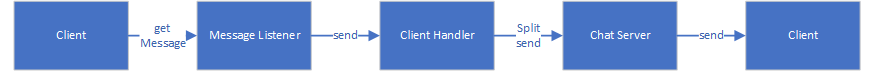
\includegraphics[width=0.8\textwidth]{img/1.png}
    \caption{程序流程图}
\end{figure}

\newpage

\subsection{实验结果}
\subsubsection{启动服务器端}
\begin{figure}[htbp]
    \centering
    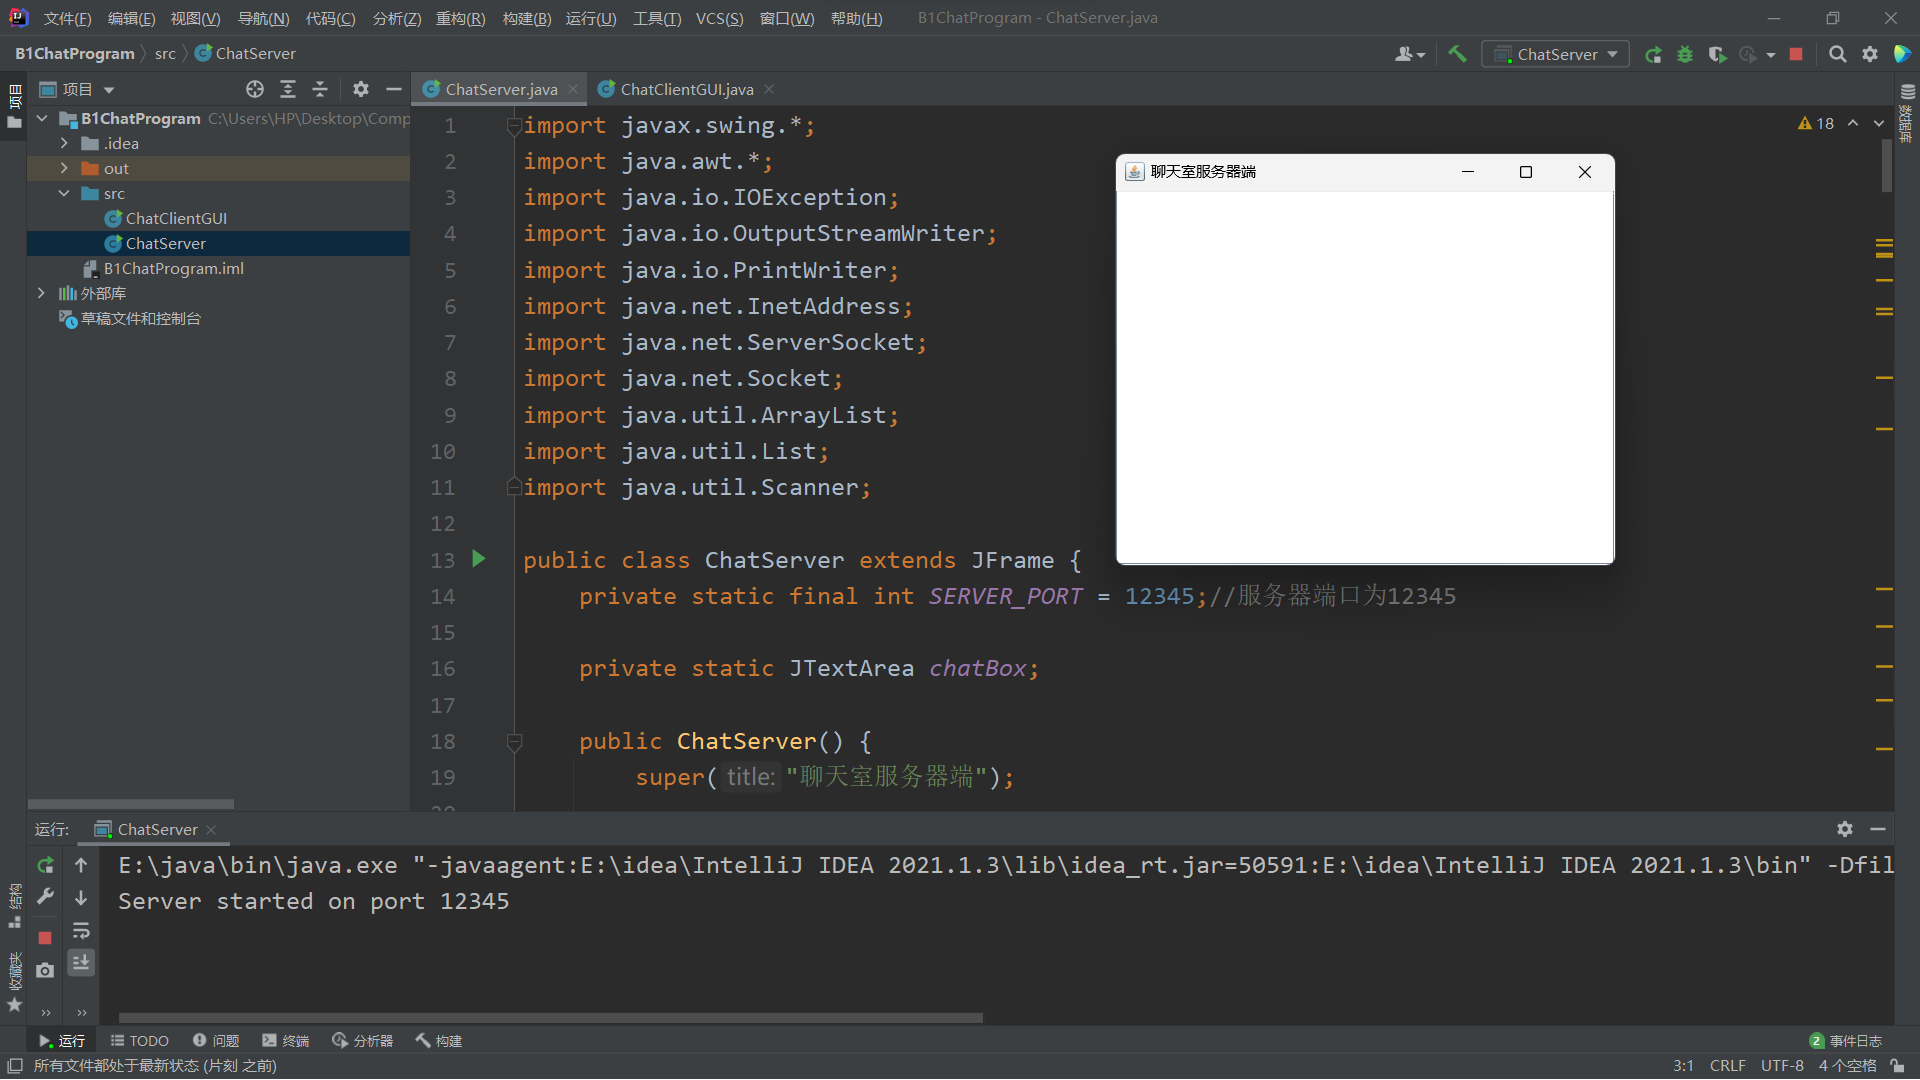
\includegraphics[width=0.8\textwidth]{img/2.png}
    \caption{启动服务器端}
\end{figure}

\subsubsection{初始化客户端}
\begin{figure}[htbp]
	\centering
	\begin{minipage}{0.3\linewidth}
		\centering
		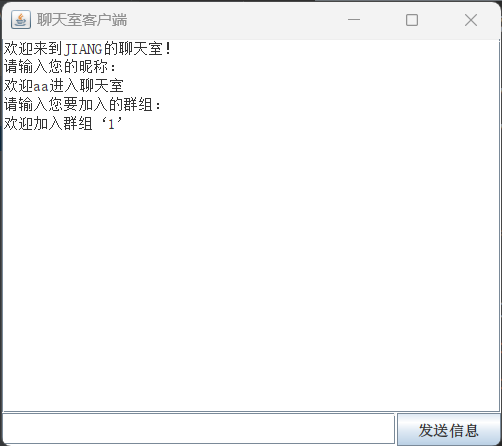
\includegraphics[width=0.9\linewidth]{img/3.png}
	\end{minipage}
	\begin{minipage}{0.3\linewidth}
		\centering
		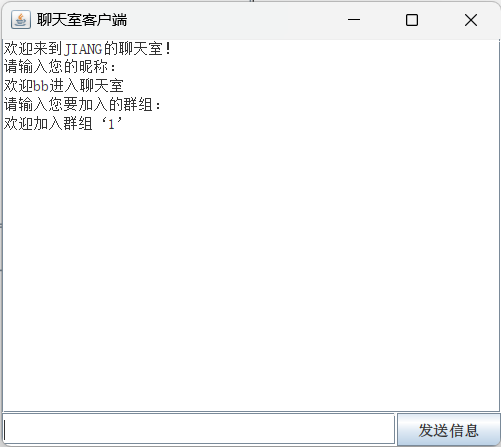
\includegraphics[width=0.9\linewidth]{img/4.png}
	\end{minipage}
	\qquad
	%让图片换行,
	
	\begin{minipage}{0.3\linewidth}
		\centering
		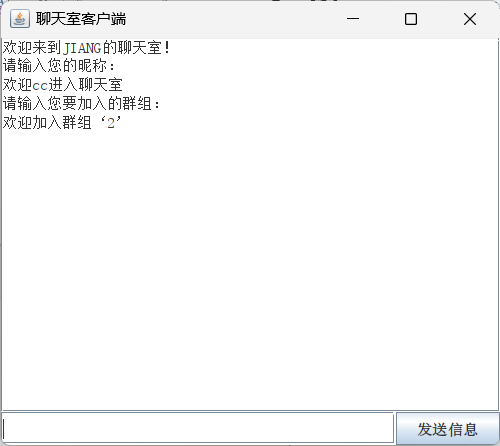
\includegraphics[width=0.9\linewidth]{img/5.png}
	\end{minipage}
	\begin{minipage}{0.3\linewidth}
		\centering
		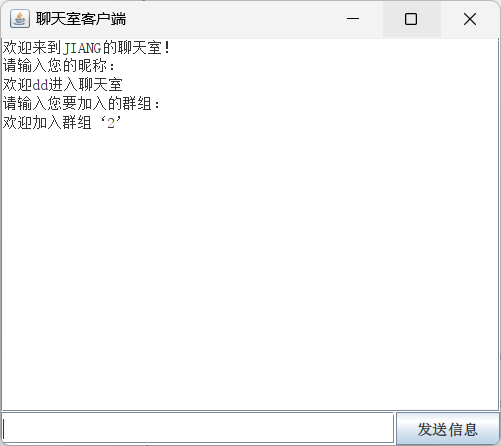
\includegraphics[width=0.9\linewidth]{img/6.png}
	\end{minipage}
\end{figure}

\subsubsection{服务器监听1}
\begin{figure}[htbp]
    \centering
    
\includegraphics[width=0.5\textwidth]{img/7.png}
    \caption{服务器监听1}
\end{figure}

\subsubsection{点对点通信}
\begin{figure}[htbp]
    \begin{minipage}{0.49\linewidth}
		\centering
		
\includegraphics[width=0.9\linewidth]{img/8.png}
	\end{minipage}
	\begin{minipage}{0.49\linewidth}
		\centering
		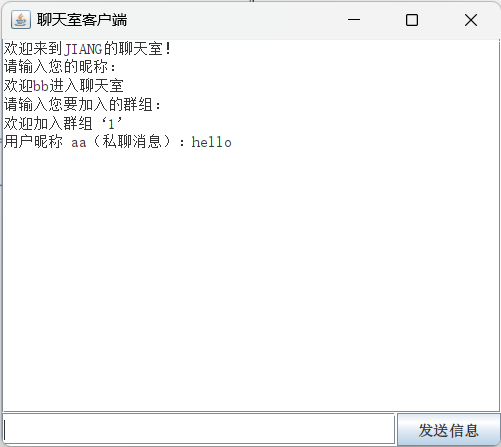
\includegraphics[width=0.9\linewidth]{img/9.png}
	\end{minipage}
\end{figure}

\newpage

\subsubsection{群组通信}
\begin{figure}[htbp]
    \begin{minipage}{0.49\linewidth}
		\centering
		
\includegraphics[width=0.9\linewidth]{img/10.png}
	\end{minipage}
	\begin{minipage}{0.49\linewidth}
		\centering
		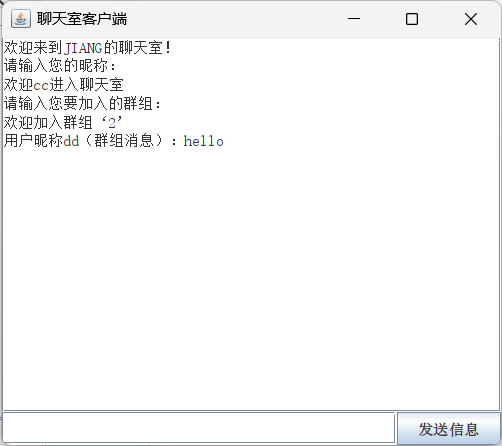
\includegraphics[width=0.9\linewidth]{img/11.png}
	\end{minipage}
\end{figure}

\subsubsection{广播通信}
\begin{figure}[htbp]
	\centering
	\begin{minipage}{0.3\linewidth}
		\centering
		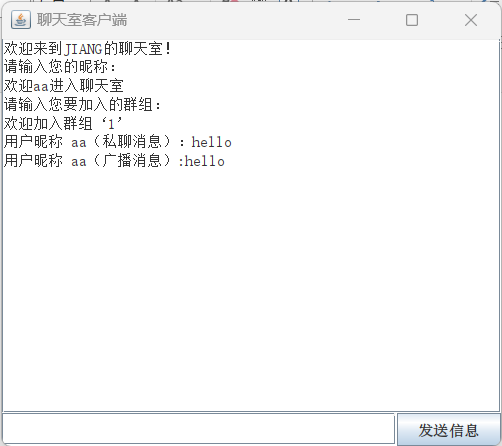
\includegraphics[width=0.9\linewidth]{img/12.png}
	\end{minipage}
	\begin{minipage}{0.3\linewidth}
		\centering
		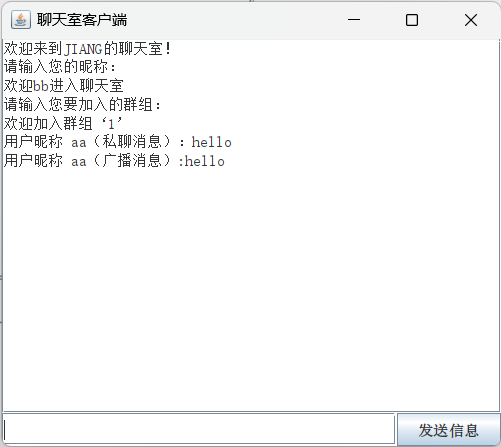
\includegraphics[width=0.9\linewidth]{img/13.png}
	\end{minipage}
	\qquad
	%让图片换行,
	
	\begin{minipage}{0.3\linewidth}
		\centering
		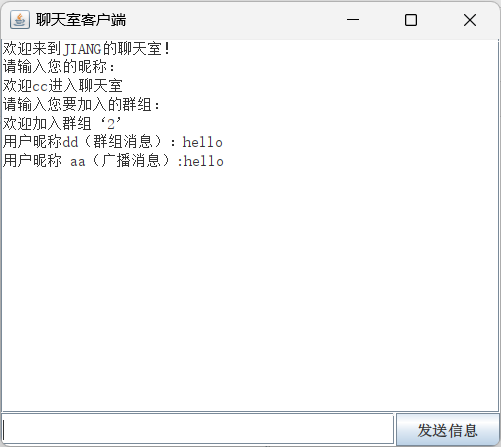
\includegraphics[width=0.9\linewidth]{img/14.png}
	\end{minipage}
	\begin{minipage}{0.3\linewidth}
		\centering
		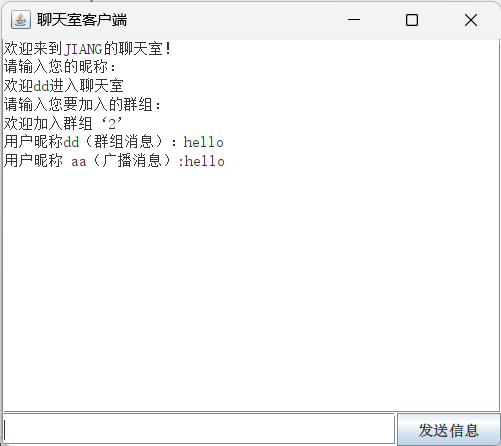
\includegraphics[width=0.9\linewidth]{img/15.png}
	\end{minipage}
\end{figure}

\newpage

\subsubsection{服务器监听2}
\begin{figure}[htbp]
    \centering
    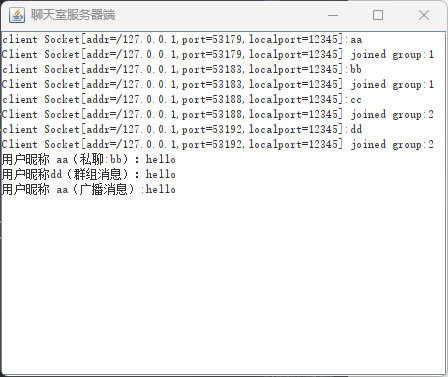
\includegraphics[width=0.5\textwidth]{img/16.png}
    \caption{服务器监听2}
\end{figure}

\section{实验设备与实验环境}
\begin{enumerate}
    \item 编程语言:Java
    \item 编程环境:IDEA,windows11操作系统
\end{enumerate}

\section{实验总结}
本次实验是实现一个简单的聊天系统,包括服务器和客户端程序的开发。通过实验,我掌握了以下内容:

Socket编程:学习了如何使用Socket建立客户端与服务器之间的通信连接,并进行数据的发送和接收。

GUI设计:使用Swing库创建了简单的用户界面,包括聊天记录显示区域和消息输入框,提供了基本的交互功能。

多线程编程:为了实现同时处理多个客户端的连接和消息交互,使用了多线程编程。每个客户端连接都在独立的线程中进行处理,避免了阻塞其他客户端的情况。

在实验过程中,遇到了一些困难和挑战:

网络通信理解:对于网络通信的概念和原理需要有一定的了解,包括服务器端的监听和客户端的连接,以及数据的发送和接收。

多线程同步:在处理多个客户端连接和消息交互时,需要注意线程之间的同步和互斥,避免数据竞争和不一致的情况。

GUI设计和事件处理:创建用户界面并处理用户的输入和操作需要熟悉Swing库的使用,并理解事件驱动的编程模型。

网络编程是实现分布式系统和实时通信的关键技术之一,了解并掌握Socket编程对于开发网络应用程序至关重要。多线程编程可以提高程序的并发性和响应性,但也带来了线程安全性的考虑,需要注意同步和互斥机制的使用。
GUI设计需要结合用户需求和交互模式,简洁明了的界面和良好的用户体验是提升应用程序质量的重要方面。在开发实时通信系统时,需要考虑网络延迟和消息丢失等因素,设计合适的机制来保证消息的可靠性和实时性。

通过实验,我加深了对网络通信和多线程编程的理解,并提升了问题解决能力和编程技巧。本次实验让我在实践中掌握了聊天系统的基本原理和实现方式,同时也面对了一些挑战和难题。通过不断的学习和实践,我逐渐提升了对网络编程和多线程编程的理解和应用能力。

\newpage

\section{附录}
\subsection{ChatServer.java源代码}
\begin{lstlisting}[title=ChatServer.java源代码,frame=shadowbox]
    import javax.swing.*;
    import java.awt.*;
    import java.io.IOException;
    import java.io.OutputStreamWriter;
    import java.io.PrintWriter;
    import java.net.InetAddress;
    import java.net.ServerSocket;
    import java.net.Socket;
    import java.util.ArrayList;
    import java.util.List;
    import java.util.Scanner;
    
    public class ChatServer extends JFrame {
        private static final int SERVER_PORT = 12345;//服务器端口为12345
    
        private static JTextArea chatBox;
    
        public ChatServer() {
            super("聊天室服务器端");
    
            chatBox = new JTextArea();
            chatBox.setEditable(false);
    
            JScrollPane jsp = new JScrollPane(chatBox);
            jsp.setPreferredSize(new Dimension(400, 300));
            chatBox.setFont(new Font("宋体", Font.PLAIN, 12));
    
            setLayout(new BorderLayout());
            add(jsp, BorderLayout.CENTER);
    
            setDefaultCloseOperation((JFrame.DISPOSE_ON_CLOSE));
            pack();
            setVisible(true);
        }
    
        private static class ClientInfo {
            private Socket socket;//客户端端口
            private String nickname;//客户端昵称
            private String groupName;//客户端组名
    
            public ClientInfo(Socket socket, String nickname, String groupName) {
                this.socket = socket;
                this.nickname = nickname;
                this.groupName = groupName;
            }
    
            public Socket getSocket() {
                return socket;
            }
    
            public String getNickname() {
                return nickname;
            }
    
            public String getGroupName() {
                return groupName;
            }
    
            public Socket getSocketByNickname(String nickname) {
                for (ClientInfo clientInfo : clientSockets) {
                    if (clientInfo.getNickname().equals(nickname)) {
                        return clientInfo.getSocket();
                    }
                }
                return null;
            }
        }
    
        private static List<ClientInfo> clientSockets = new ArrayList<>();
    
        private static class ClientHandler implements Runnable {
            private Socket clientSocket;
            private PrintWriter writer;
    
            public String Name;
            public String GroupName;
    
            public ClientHandler(Socket clientSocket) {
                this.clientSocket = clientSocket;
            }
    
            public void appendMessage(String message) {
                SwingUtilities.invokeLater(new Runnable() {
                    @Override
                    public void run() {
                        chatBox.append(message + "\n");
                    }
                });
            }
    
            @Override
            public void run() {
                try {
                    Scanner scanner = new Scanner(clientSocket.getInputStream(), "UTF-8");//获取客户端的请求
                    writer = new PrintWriter(new OutputStreamWriter(clientSocket.getOutputStream(), "UTF-8"), true);//向客户端发送信息
    
                    writer.println("欢迎来到JIANG的聊天室!");
    
                    writer.println("请输入您的昵称:");
                    Name = scanner.nextLine();
                    writer.println("欢迎" + Name + "进入聊天室");
    
                    System.out.println("client " + clientSocket + ":" + Name);
                    appendMessage("client " + clientSocket + ":" + Name);
    
                    writer.println("请输入您要加入的群组:");
                    GroupName = scanner.nextLine();
                    writer.println("欢迎加入群组‘" + GroupName + "’");
    
                    System.out.println("Client " + clientSocket + " joined group:" + GroupName);
                    appendMessage("Client " + clientSocket + " joined group:" + GroupName);
    
                    ClientInfo clientInfo = new ClientInfo(clientSocket, Name, GroupName);
                    clientSockets.add(clientInfo);
    
                    //进行消息发送方式的分离
                    while (true) {
                        String message = scanner.nextLine();
                        if (message.startsWith("@p")) {
                            handlePersonToPersonMessage(message);
                        } else if (message.startsWith("@g")) {
                            handleGroupMessage(message, GroupName);
                        } else if (message.startsWith("@b")) {
                            handleBroadcastMessage(message);
                        } else {
                            System.out.println("Received message from " + Name + ":" + message);
                            sendToAllClients("用户昵称" + Name + ":" + message);
                            appendMessage("用户昵称" + Name + ":" + message);
                        }
                    }
                } catch (IOException e) {//捕获输入输出操作过程中可能发生的异常情况,例如文件读写错误、网络连接问题
                    e.printStackTrace();
                } finally {
                    clientSockets.remove(clientSocket);
                    System.out.println("Client " + clientSocket + " disconnected");
                    sendToAllClients("Client " + clientSocket + " disconnected");
                }
            }
    
            private void handlePersonToPersonMessage(String message) {
                String[] parts = message.split(" ", 3);//将消息切成三片,分别是报头、接收者及消息内容
                if (parts.length == 3) {
                    String receiver = parts[1];
                    String p2pMessage = parts[2];
    
                    System.out.println("Received Person-to-Person message from " + Name + " to " + receiver + ":" + p2pMessage);
                    sendPersonToPerson(receiver, "用户昵称 " + Name + "(私聊消息):" + p2pMessage);
                    sendPersonToPerson(Name, "用户昵称 " + Name + "(私聊消息):" + p2pMessage);
                    appendMessage("用户昵称 " + Name + "(私聊:" + receiver + "):" + p2pMessage);
                }
            }
    
            private void handleGroupMessage(String message, String groupName) {
                String[] parts = message.split(" ", 2);
                if (parts.length == 2) {
                    String groupMessage = parts[1];
    
                    System.out.println("Received group message from " + Name + "(group:" + groupName + "):" + groupMessage);
                    sendToGroup(groupName, "用户昵称" + Name + "(群组消息):" + groupMessage);
                    appendMessage("用户昵称" + Name + "(群组消息):" + groupMessage);
                }
            }
    
            private void handleBroadcastMessage(String message) {
                String[] parts = message.split(" ", 2);
                if (parts.length == 2) {
                    String broadcastMessage = parts[1];
    
                    System.out.println("Received broadcast message from " + Name + ":" + broadcastMessage);
                    sendToAllClients("用户昵称 " + Name + "(广播消息):" + broadcastMessage);
                    appendMessage("用户昵称 " + Name + "(广播消息):" + broadcastMessage);
                }
            }
    
            private void sendToAllClients(String message) {
                for (ClientInfo clientInfo : clientSockets) {
                    try {//向所有客户端输出消息
                        //通过clientInfo.getSocket().getOutputStream()获取客户端的输出流,
                        //使用OutputStreamWriter和指定的字符编码(UTF-8)创建PrintWriter对象socketWriter,用于向客户端发送消息。
                        //使用socketWriter.println(message)将message发送给客户端
                        PrintWriter socketWriter = new PrintWriter(new OutputStreamWriter(clientInfo.getSocket().getOutputStream(), "UTF-8"), true);
                        socketWriter.println(message);
                    } catch (IOException e) {
                        e.printStackTrace();
                    }
                }
            }
    
            private void sendToGroup(String groupName, String message) {
                for (ClientInfo clientInfo : clientSockets) {
                    if (clientInfo.getGroupName().equals(groupName)) {
                        try {
                            PrintWriter socketWriter = new PrintWriter(new OutputStreamWriter(clientInfo.getSocket().getOutputStream(), "UTF-8"), true);
                            socketWriter.println(message);
                        } catch (IOException e) {
                            e.printStackTrace();
                        }
                    }
                }
            }
    
            private void sendPersonToPerson(String targetName, String message) {
                for (ClientInfo clientInfo : clientSockets) {
                    if (clientInfo.getNickname().equals(targetName)) {
                        try {
                            PrintWriter socketWriter = new PrintWriter(new OutputStreamWriter(clientInfo.getSocket().getOutputStream(), "UTF-8"), true);
                            socketWriter.println(message);
                            break;
                        } catch (IOException e) {
                            e.printStackTrace();
                        }
                    }
                }
            }
        }
    
        public static void main(String[] args) {
            SwingUtilities.invokeLater(new Runnable() {
                @Override
                public void run() {
                    new ChatServer();
                }
            });
    
            try {
                //创建一个ServerSocket对象,将其绑定到指定的服务器端口和本地地址
                //ServerSocket是java实现服务器端的套接字,监听指定的端口,接收客户端连接请求,并与客户端进行通信
                //SERVER_PORT是服务器绑定端口,为12345
                //backlog设为0表示使用默认值,即系统根据具体实现来选择一个合适的默认队列长度
                //InetAddress.getByName("localhost")获取本机IP
                ServerSocket serverSocket = new ServerSocket(SERVER_PORT, 0, InetAddress.getByName("localhost"));
    
                System.out.println("Server started on port " + SERVER_PORT);
    
                while (true) {
                    //serverSocket.accept()方法是一个阻塞调用,意味着程序会在此处暂停,直到有客户端请求连接才会继续执行。
                    Socket clientSocket = serverSocket.accept();
    
                    System.out.println("New client connected in " + clientSocket);
                    //创建了一个新的线程clientThread,并将其与客户端的连接clientSocket关联。
                    // 通过start()方法启动线程后,线程将执行ClientHandler对象中定义的任务
                    Thread clientThread = new Thread(new ClientHandler(clientSocket));
                    clientThread.start();
                }
            } catch (IOException e) {
                e.printStackTrace();
            }
        }
    }        
\end{lstlisting}

\subsection{ChatClientGUI.java源代码}
\begin{lstlisting}[title=ChatClientGUI.java源代码,frame=shadowbox]
    import javax.swing.*;
    import java.awt.*;
    import java.awt.event.ActionEvent;
    import java.awt.event.ActionListener;
    import java.io.*;
    import java.net.*;
    import java.util.*;
    
    public class ChatClientGUI extends JFrame {
        private static final String SERVER_HOST = "localhost";//服务器地址
        private static final int SERVER_PORT = 12345;//服务器端口
    
        private Socket socket;//客户端套接字
        private PrintWriter writer;//输出流
        private Scanner scanner;
    
        private JTextArea chatBox;//聊天框
        private JTextField messageField;//消息输入框
    
        public ChatClientGUI() {
            super("聊天室客户端");
    
            chatBox = new JTextArea();
            chatBox.setEditable(false);//设置为不可编辑
    
            JScrollPane jsp = new JScrollPane(chatBox);
            jsp.setPreferredSize(new Dimension(400, 300));
            chatBox.setFont(new Font("宋体", Font.PLAIN, 12));
    
            messageField = new JTextField();
            messageField.addActionListener(new ActionListener() {
                @Override
                public void actionPerformed(ActionEvent e) {
                    sendMessage(messageField.getText());
                }
            });
    
            JButton send = new JButton("发送信息");
            send.addActionListener(new ActionListener() {
                @Override
                public void actionPerformed(ActionEvent e) {
                    sendMessage(messageField.getText());
                }
            });
    
            JPanel input = new JPanel();
            input.setLayout(new BorderLayout());
            input.add(messageField, BorderLayout.CENTER);
            input.add(send, BorderLayout.EAST);
    
            setLayout(new BorderLayout());
            add(jsp, BorderLayout.CENTER);
            add(input, BorderLayout.SOUTH);
    
            setDefaultCloseOperation((JFrame.DISPOSE_ON_CLOSE));
            pack();
            setVisible(true);
    
            connectToServer();
    
        }
    
        private void connectToServer() {
            try {
                //通过socket连接服务器端口
                socket = new Socket(SERVER_HOST, SERVER_PORT);
                writer = new PrintWriter(new OutputStreamWriter(socket.getOutputStream(), "UTF-8"), true);
                scanner = new Scanner(new InputStreamReader(socket.getInputStream(), "UTF-8"));
    
                //初始欢迎
                String welcomeMessage = scanner.nextLine();
                appendMessage(welcomeMessage);
    
                Thread messageListener = new Thread(new MessageListener());//创建一个新的线程来监听消息
                messageListener.start();
            } catch (IOException e) {
                e.printStackTrace();
            }
        }
    
        private void sendMessage(String message) {//发送消息并清空输入框
            writer.println(message);
            ;
            messageField.setText("");
        }
    
        private void appendMessage(String message) {//在消息框中进行消息追加
            SwingUtilities.invokeLater(new Runnable() {
                @Override
                public void run() {
                    chatBox.append(message + "\n");
                }
            });
        }
    
    
        private class MessageListener implements Runnable {
            @Override
            //使用一个无限循环来持续监听消息。
            // 通过scanner.nextLine()从输入流中读取下一行消息,并将该消息传递给appendMessage方法,以将其追加到聊天区域。
            public void run() {
                try {
                    while (true) {
                        String message = scanner.nextLine();
                        appendMessage(message);
                    }
                } catch (Exception e) {
                    e.printStackTrace();
                } finally {
                    try {
                        socket.close();
                        ;
                    } catch (IOException e) {
                        e.printStackTrace();
                    }
                }
            }
    
        }
    
        public static void main(String[] args) {
            SwingUtilities.invokeLater(new Runnable() {
                @Override
                public void run() {
                    new ChatClientGUI();
                }
            });
        }
    }
    
\end{lstlisting}

\end{document}